\documentclass[aspectratio=169]{beamer}
\usetheme{Madrid}
\usecolortheme{seahorse}
\setbeamertemplate{navigation symbols}{}
\setbeamertemplate{footline}[frame number]

\usepackage{amsmath,amssymb,bm,booktabs}
\usepackage{graphicx}
\usepackage{array}
\usepackage{mathtools}
\usepackage{tikz}
\usetikzlibrary{arrows.meta,positioning,calc}
\graphicspath{{assets/}}

\newcommand{\ket}[1]{\lvert #1\rangle}
\newcommand{\braket}[2]{\langle #1 \mid #2 \rangle}

\title{Why IDQNN Fails on Handwritten Digits}
\subtitle{A First Diagnostic Draft}
\author{}
\institute{Quantum Machine Learning}
\date{\today}

\begin{document}

\begin{frame}
  \titlepage
\end{frame}

% \begin{frame}{Working Hypothesis}
%   \begin{itemize}
%     \item The test-time output is almost uninformative.
%     \item The induced probability laws are highly special, not generic image distributions.
%     \item Only CZ-connected active qubits share correlations; many bits remain $50/50$ in the $X$ basis.
%   \end{itemize}
% \end{frame}

\begin{frame}{IDQNN Structure}
  \begin{columns}[T,onlytextwidth]
    \begin{column}{0.47\textwidth}
      \centering
      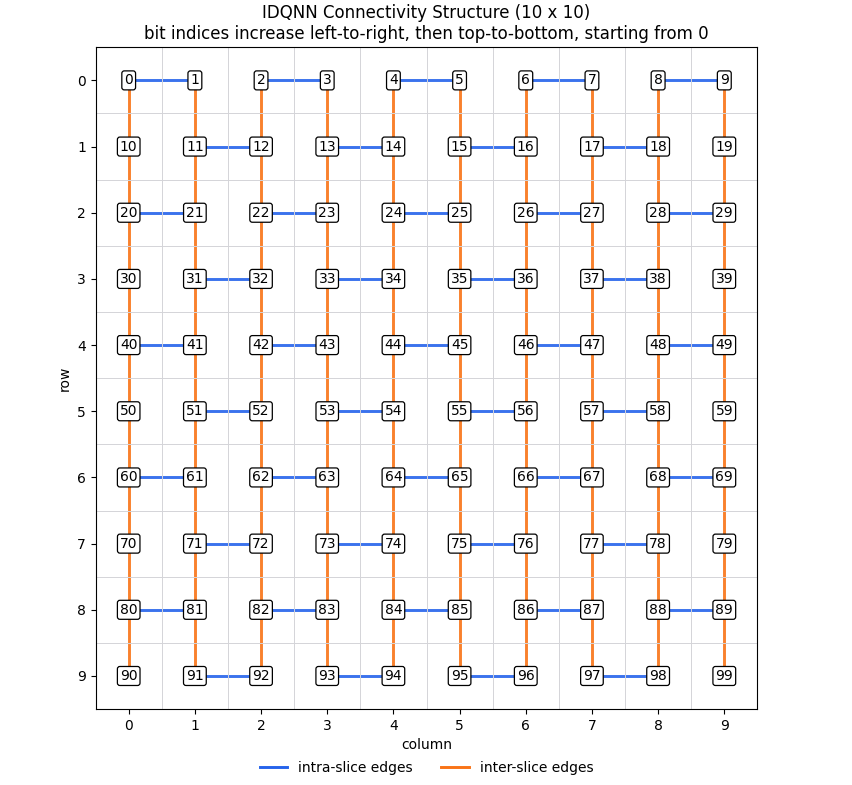
\includegraphics[width=0.9\textwidth,height=0.72\textheight,keepaspectratio]{IDQNN_structure.png}

      \vspace{0.4em}
      \footnotesize
      Nearest-neighbor CZ structure on the $10\times10$ bit grid.
    \end{column}
    \begin{column}{0.50\textwidth}
      \centering
      \resizebox{0.98\linewidth}{!}{%
      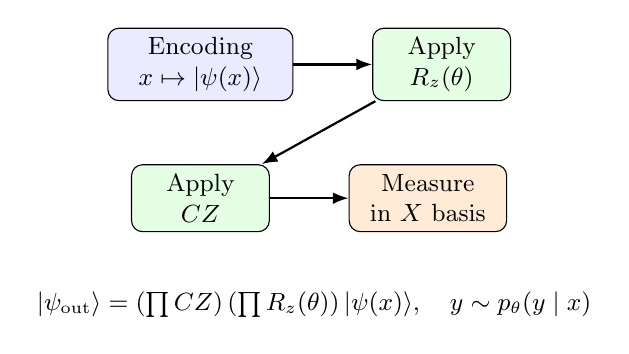
\begin{tikzpicture}[
        font=\small,
        node distance=8mm and 10mm,
        box/.style={draw, rounded corners, minimum width=2.35cm, minimum height=0.85cm, align=center, fill=blue!8},
        op/.style={draw, rounded corners, minimum width=1.75cm, minimum height=0.85cm, align=center, fill=green!10},
        meas/.style={draw, rounded corners, minimum width=2.0cm, minimum height=0.85cm, align=center, fill=orange!16},
        arrow/.style={-{Latex[length=2mm]}, thick}
      ]
        \node[box] (enc) {Encoding\\$x\mapsto \ket{\psi(x)}$};
        \node[op, right=of enc] (rz) {Apply\\$R_z(\theta)$};
        \node[op, below=of enc] (cz) {Apply\\$CZ$};
        \node[meas, right=of cz] (mx) {Measure\\in $X$ basis};

        \draw[arrow] (enc) -- (rz);
        \draw[arrow] (rz) -- (cz);
        \draw[arrow] (cz) -- (mx);

        \node[align=center] at ($(cz)!0.5!(mx)+(0,-1.35)$)
        {$\ket{\psi_{\mathrm{out}}}=\left(\prod CZ\right)\left(\prod R_z(\theta)\right)\ket{\psi(x)},\quad y\sim p_\theta(y\mid x)$};
      \end{tikzpicture}%
      }
      White pixels(1) are encoded to $\ket{0}$, black pixels(0) to $\ket{+}$. 
      
      Generate the corresponding y bits by measuring the qubits.
    \end{column}
  \end{columns}
\end{frame}

\begin{frame}{Test Sample \#99: Distance between Output and Label-Diagonal Encoding}
  \small
  \centering
  10000 test-time samples for \#99 are generated and averaged.

  \vfill
  \begin{columns}[c,onlytextwidth]
    \begin{column}{0.48\textwidth}
      \centering
      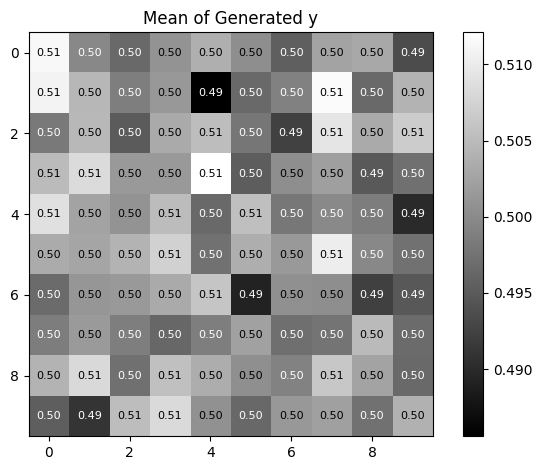
\includegraphics[width=\textwidth,height=0.63\textheight,keepaspectratio]{output_of_testbitstring_99_10000avg.png}
    \end{column}
    \begin{column}{0.48\textwidth}
      \centering
      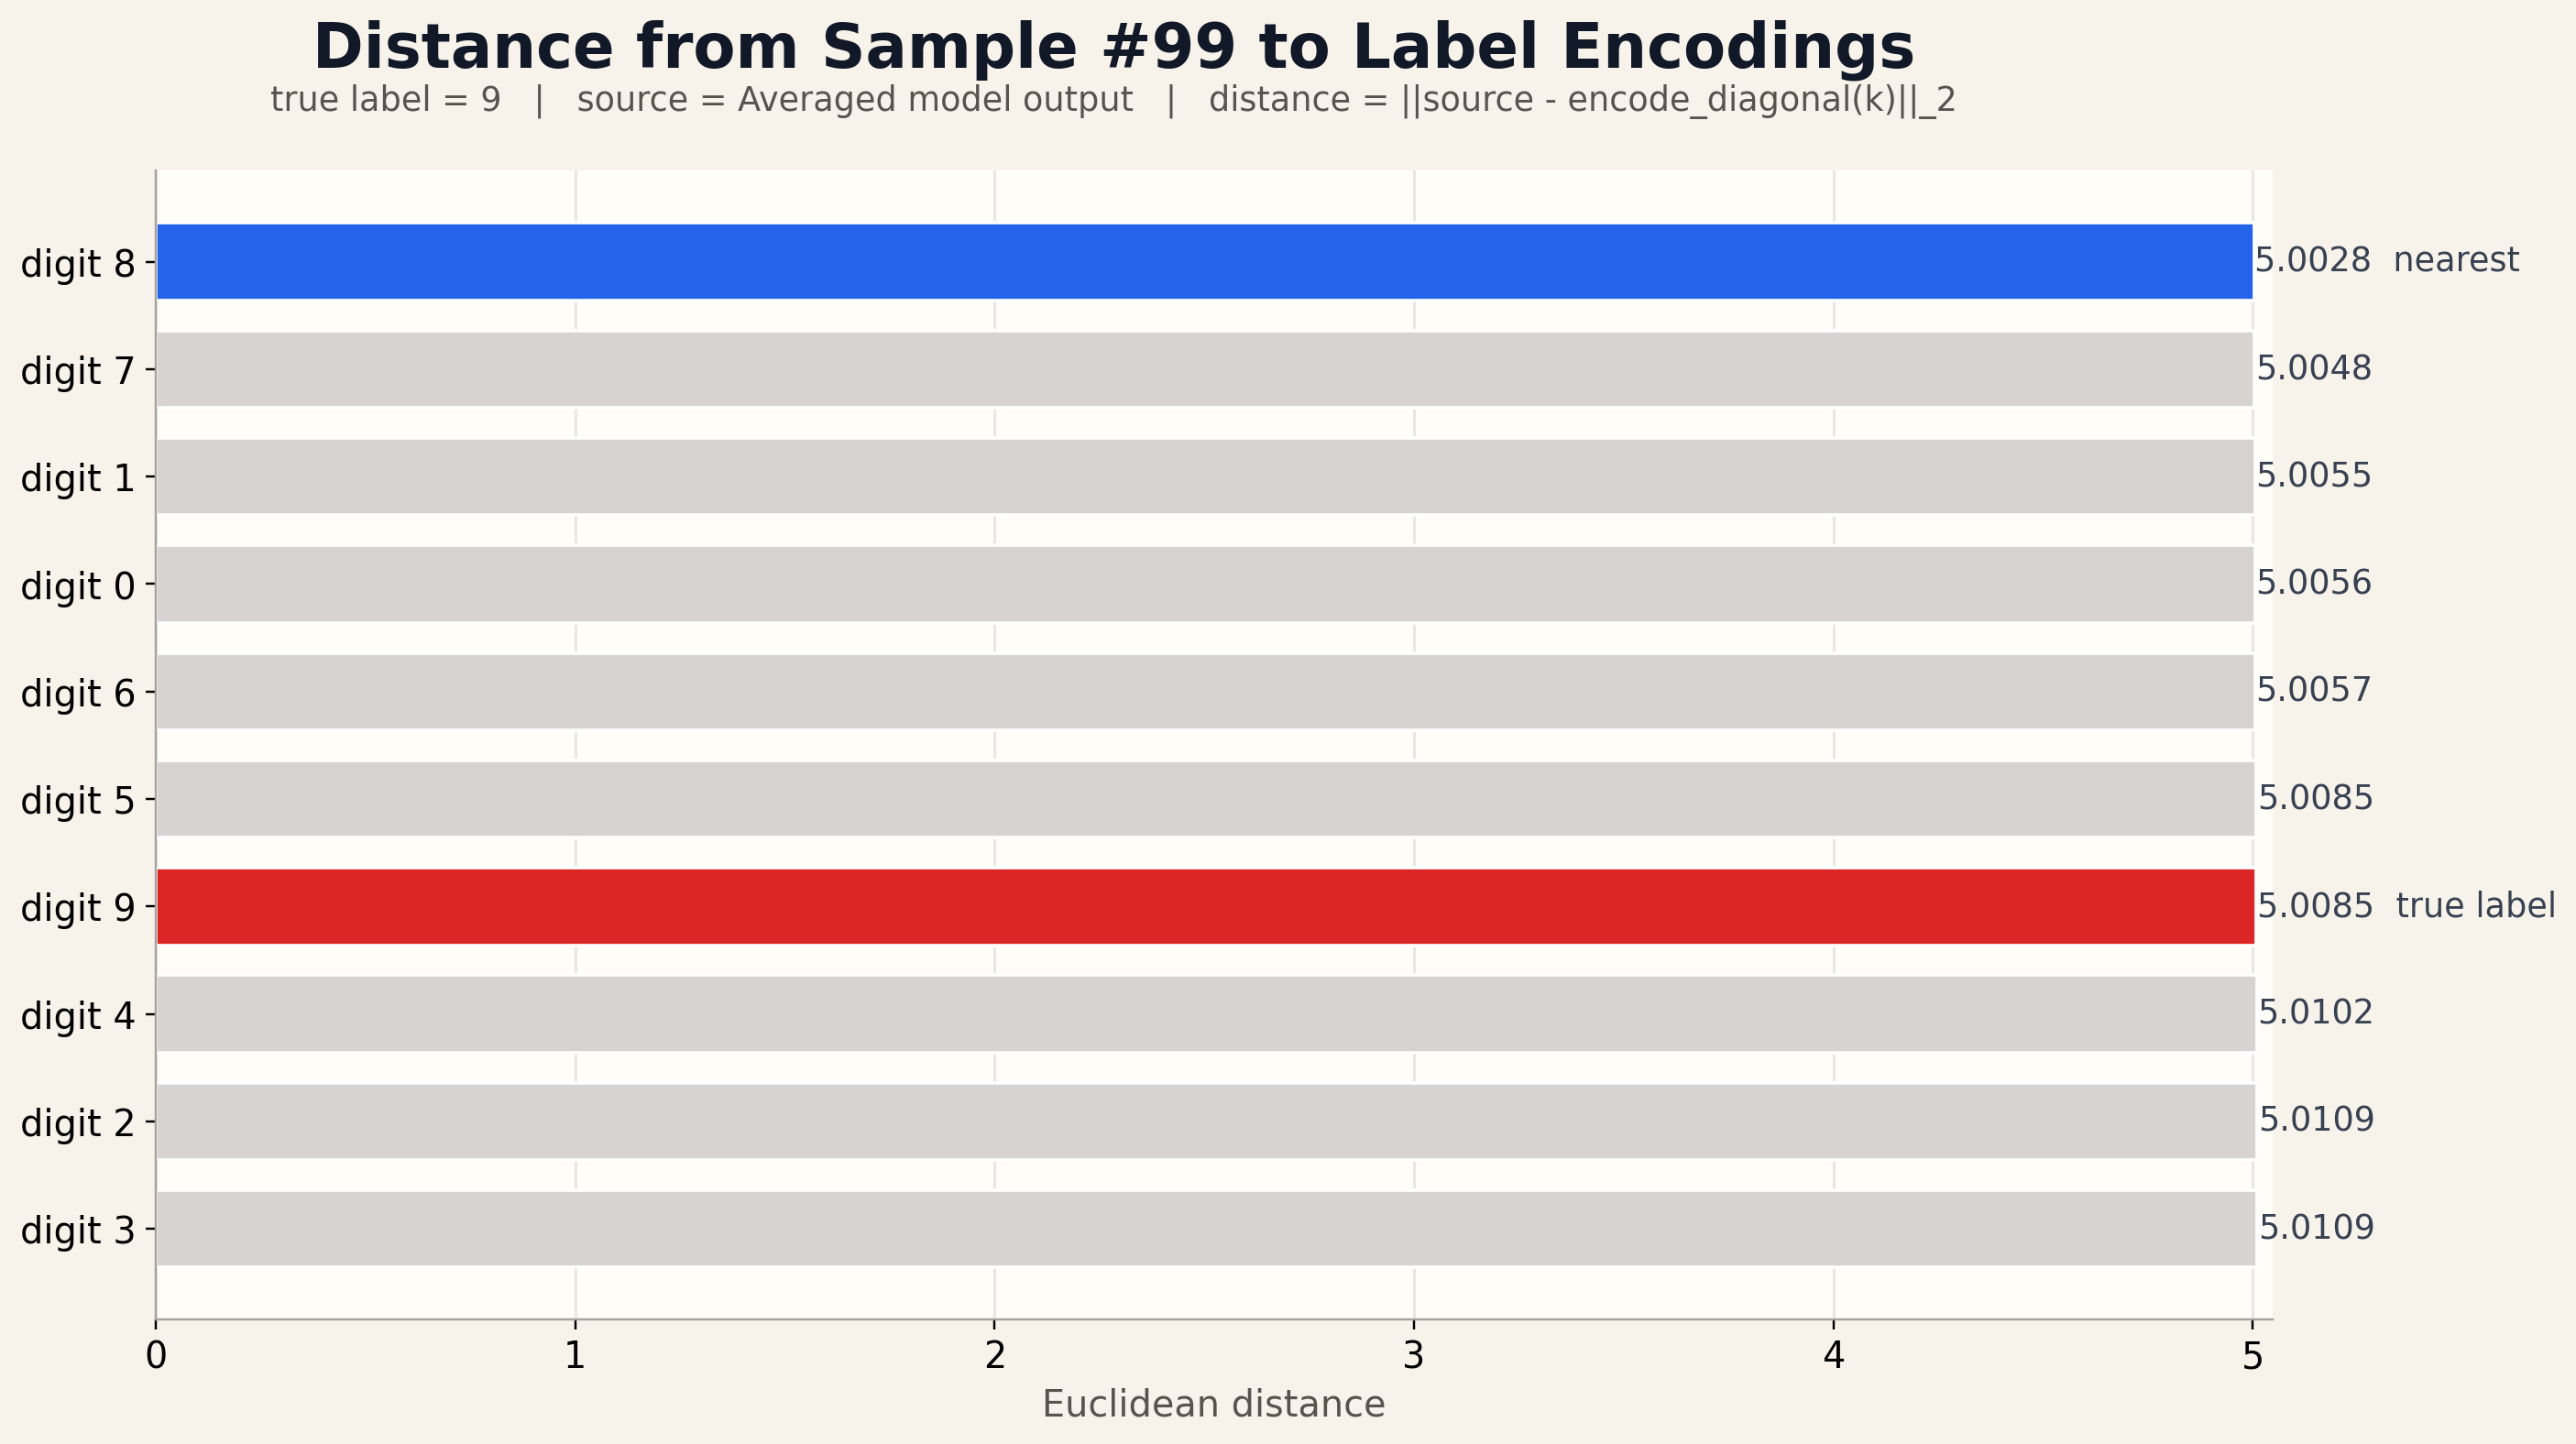
\includegraphics[width=\textwidth,height=0.63\textheight,keepaspectratio]{distance_bars_sample_99_generated_mean_threshold_0_4.png}
    \end{column}
  \end{columns}

  \vspace{0.3em}
  \footnotesize
  The nearest label for sample \#99 is digit 8 rather than the true label 9.
  \vfill
\end{frame}

\begin{frame}{ Test Sample \#99: output distribution structure}
  \centering
  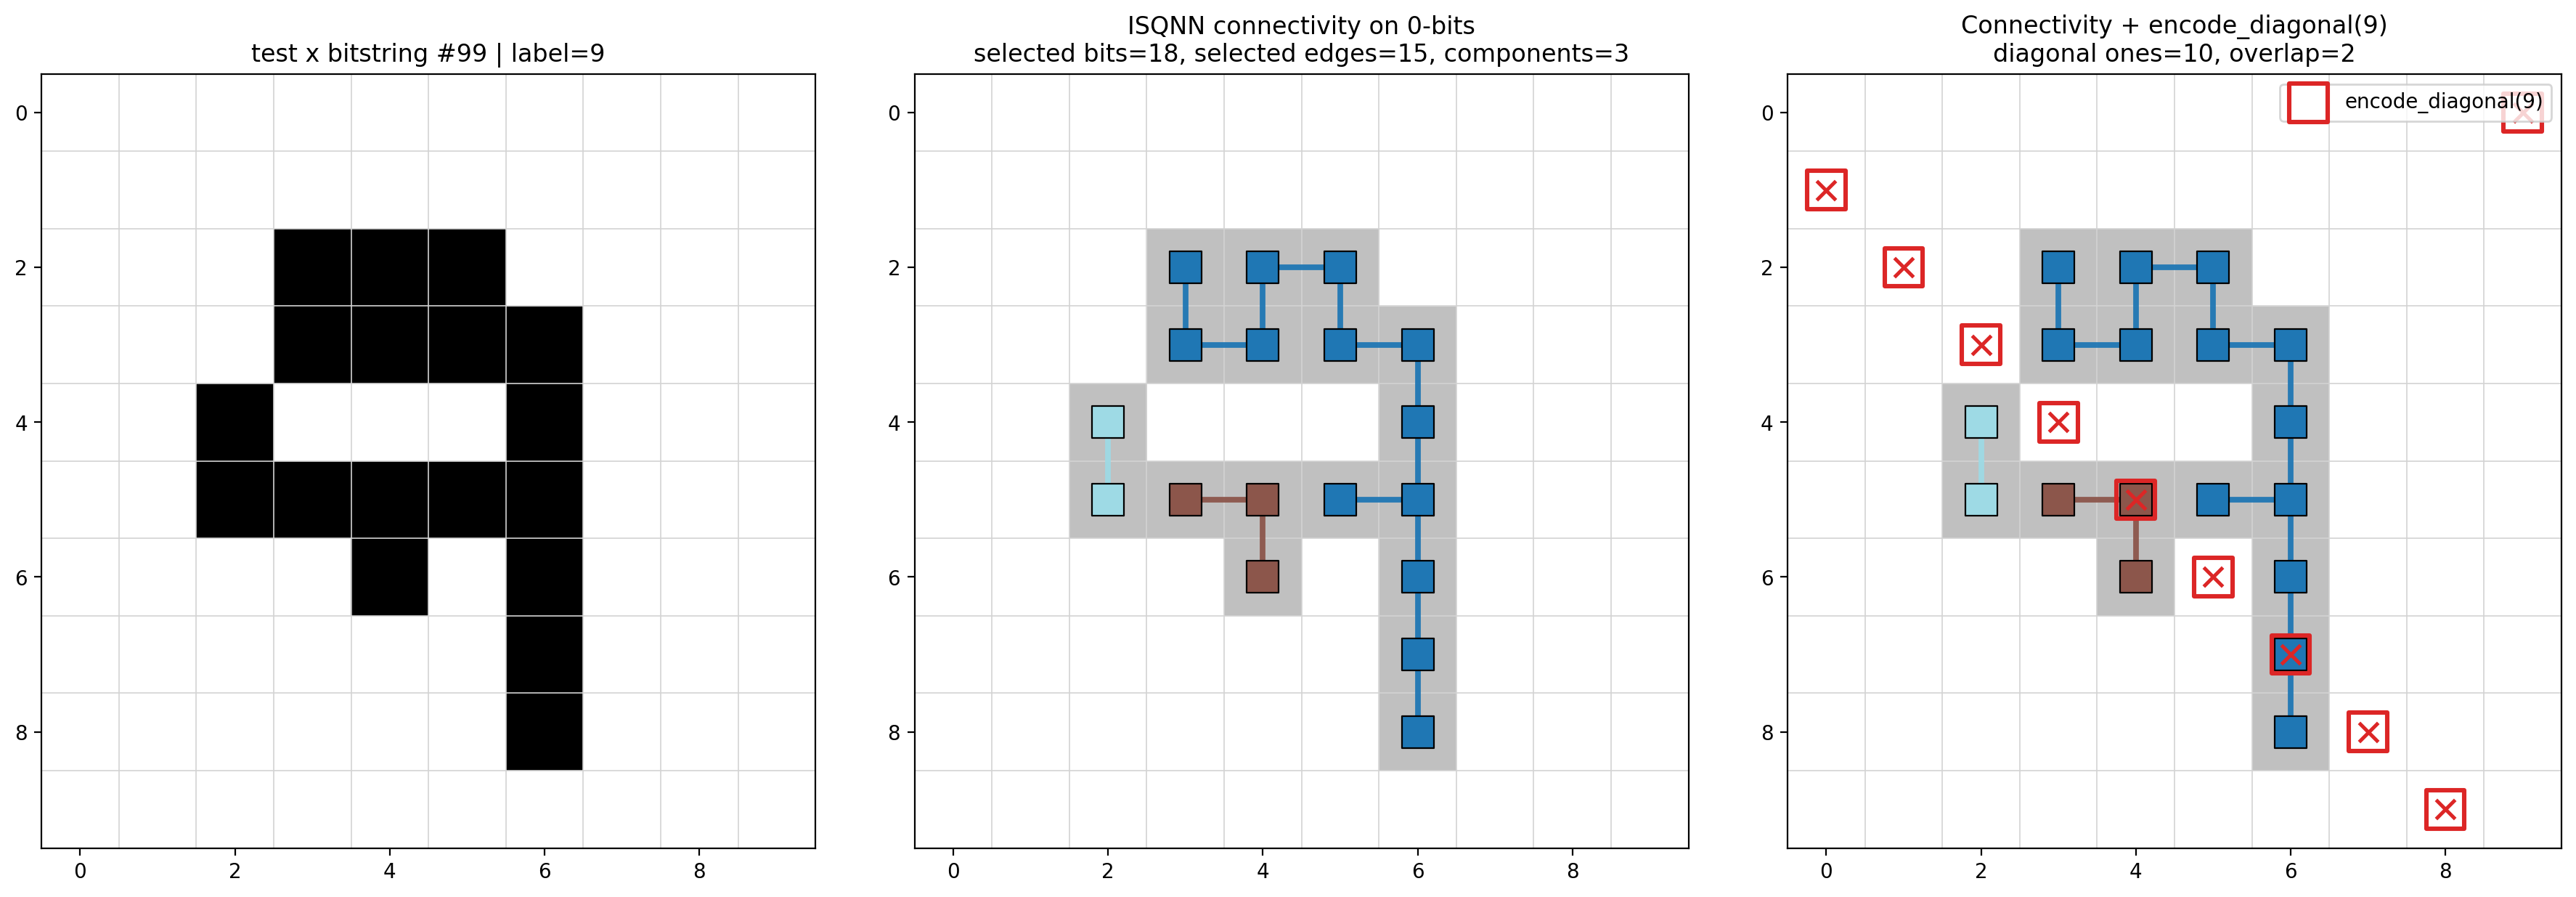
\includegraphics[width=0.96\textwidth,height=0.78\textheight,keepaspectratio]{mnist_test_99_connectivity_label_9.png}

  \vspace{0.25em}
  \footnotesize
  \begin{itemize}
    \item Measurement outcomes of White pixels are always $50/50$ .
    \item overlap with the label-diagonal encoding is very limited.
  \end{itemize}
\end{frame}

\begin{frame}{Outputs distributions for black pixels blocks:}
  \scriptsize
  \begin{columns}[T,onlytextwidth]
    \begin{column}{0.38\textwidth}
      \begin{minipage}[t][0.23\textheight][t]{\linewidth}
        \begin{block}{\texttt{101}}
          \[
            \ket{0}\ket{+}\ket{0}
          \]
          $$ \ket{0}
          \left(
            \ket{+}\cos\frac{\theta_2}{2}
            -
            i\ket{-}\sin\frac{\theta_2}{2}
          \right)
          \ket{0}.$$
          \[
            P(y_2=0)=\cos^2\frac{\theta_2}{2},
            \quad
            P(y_2=1)=\sin^2\frac{\theta_2}{2}
          \]
          \[
            y_1,y_3:\;50/50
          \]
        \end{block}
      \end{minipage}

      \vspace{0.45em}

      \begin{minipage}[t][0.46\textheight][t]{\linewidth}
        \begin{block}{\texttt{1001}}
          \[
            \ket{0}\ket{+}\ket{+}\ket{0}
          \]
          \[
            P(m_2,m_3)=\frac14\left(1+m_2m_3\sin\theta_2\sin\theta_3\right)
          \]
          \[
            P(++)=P(--)=\frac14\left(1+\sin\theta_2\sin\theta_3\right)
          \]
          \[
            P(+-)=P(-+)=\frac14\left(1-\sin\theta_2\sin\theta_3\right)
          \]
        \end{block}
      \end{minipage}
    \end{column}

    \begin{column}{0.60\textwidth}
      \begin{minipage}[t][0.72\textheight][t]{\linewidth}
        \begin{block}{\texttt{10001}}
          \[
            \ket{0}\ket{+}\ket{+}\ket{+}\ket{0}
          \]
          \[
            P(m_2,m_3,m_4)
            =
            \frac18\left[
              1+m_2m_4\cos\theta_2\cos\theta_4
              -m_2m_3m_4\cos\theta_3\sin\theta_2\sin\theta_4
            \right]
          \]
          \[
            m_j=
            \begin{cases}
              +1,& \ket{+}\\
              -1,& \ket{-}
            \end{cases}
          \]

          \vspace{0.4em}
          \begin{itemize}
            \item \texttt{101}: one tunable internal bit.
            \item \texttt{1001}: pairwise correlation appears.
            \item \texttt{10001}: higher-order but still local correlation.
            \item Outer qubits measurements outcomes remain $50/50$ in the $X$ basis.
          \end{itemize}
        \end{block}
      \end{minipage}
    \end{column}
  \end{columns}
\end{frame}


% \begin{frame}{Case A: Pattern \texttt{101}}
%   \small
%   \[
%     \ket{\psi_{\mathrm{enc}}}=\ket{0}\ket{+}\ket{0},
%     \qquad
%     U=\mathrm{CZ}_{12}\mathrm{CZ}_{23}\prod_{j=1}^{3}R_z(\theta_j).
%   \]

%   \[
%     U\ket{\psi_{\mathrm{enc}}}
%     =
%     e^{-i(\theta_1+\theta_3)/2}
%     \ket{0}
%     \left(
%       \ket{+}\cos\frac{\theta_2}{2}
%       -
%       i\ket{-}\sin\frac{\theta_2}{2}
%     \right)
%     \ket{0}.
%   \]

%   \[
%     P(y_2=0)=\cos^2\frac{\theta_2}{2},
%     \qquad
%     P(y_2=1)=\sin^2\frac{\theta_2}{2}.
%   \]

%   \vspace{0.2em}
%   \footnotesize
%   Only $\theta_2$ survives. The first and third measured bits stay $50/50$ in the $X$ basis.
% \end{frame}

% \begin{frame}{Case B: Pattern \texttt{1001}}
%   \scriptsize
%   \[
%     \ket{\psi_{R}}
%     =
%     \ket{0}
%     \left(
%       \ket{+}\cos\frac{\theta_2}{2}
%       -
%       i\ket{-}\sin\frac{\theta_2}{2}
%     \right)
%     \left(
%       \ket{+}\cos\frac{\theta_3}{2}
%       -
%       i\ket{-}\sin\frac{\theta_3}{2}
%     \right)
%     \ket{0}.
%   \]

%   \[
%     \mathrm{CZ}_X
%     =
%     \frac{1}{2}
%     \begin{pmatrix}
%       1 & 1 & 1 & -1 \\
%       1 & 1 & -1 & 1 \\
%       1 & -1 & 1 & 1 \\
%       -1 & 1 & 1 & 1
%     \end{pmatrix}.
%   \]

%   \[
%   \begin{aligned}
%     \ket{\psi_{\mathrm{out}}}
%     = \frac{1}{2} \Big[
%     &\left( \cos \frac{\theta_2 - \theta_3}{2} - i \sin \frac{\theta_2 + \theta_3}{2} \right) \ket{++} \\
%     +&\left( \cos \frac{\theta_2 + \theta_3}{2} + i \sin \frac{\theta_2 - \theta_3}{2} \right) \ket{+-} \\
%     +&\left( \cos \frac{\theta_2 + \theta_3}{2} - i \sin \frac{\theta_2 - \theta_3}{2} \right) \ket{-+} \\
%     -&\left( \cos \frac{\theta_2 - \theta_3}{2} + i \sin \frac{\theta_2 + \theta_3}{2} \right) \ket{--}
%     \Big].
%   \end{aligned}
%   \]

%   \[
%     P(++)=P(--)=\frac{1}{4}\left(1+\sin\theta_2\sin\theta_3\right),
%     \quad
%     P(+-)=P(-+)=\frac{1}{4}\left(1-\sin\theta_2\sin\theta_3\right).
%   \]
% \end{frame}

% \begin{frame}{Case C: Pattern \texttt{10001}}
%   \small
%   \[
%     \ket{\psi_R}
%     =
%     \ket{0}
%     \prod_{j=2}^{4}
%     \left(
%       \ket{+}\cos\frac{\theta_j}{2}
%       -
%       i\ket{-}\sin\frac{\theta_j}{2}
%     \right)
%     \ket{0}.
%   \]

%   Let $m_j=+1$ for $\ket{+}$ and $m_j=-1$ for $\ket{-}$ in the $X$ basis. After the nontrivial CZ gates,
%   \[
%     P(m_2,m_3,m_4)
%     =
%     \frac{1}{8}
%     \left[
%       1
%       +
%       m_2m_4\cos\theta_2\cos\theta_4
%       -
%       m_2m_3m_4\cos\theta_3\sin\theta_2\sin\theta_4
%     \right].
%   \]

%   \vspace{0.2em}
%   \footnotesize
%   The outer parameters couple to each other, while the middle qubit only modulates that coupling through $\cos\theta_3$.
% \end{frame}

% \begin{frame}{With More CZ-Connected Qubits}
%   \begin{itemize}
%     \item The formula becomes more complicated, but not arbitrary.
%     \item Correlations are still generated by connected CZ blocks.
%     \item This is a strong structural bias: the model does not freely explore generic $10\times10$ image distributions.
%   \end{itemize}
% \end{frame}


\begin{frame}{Connectivity Example: Test Sample \#157}
  \centering
  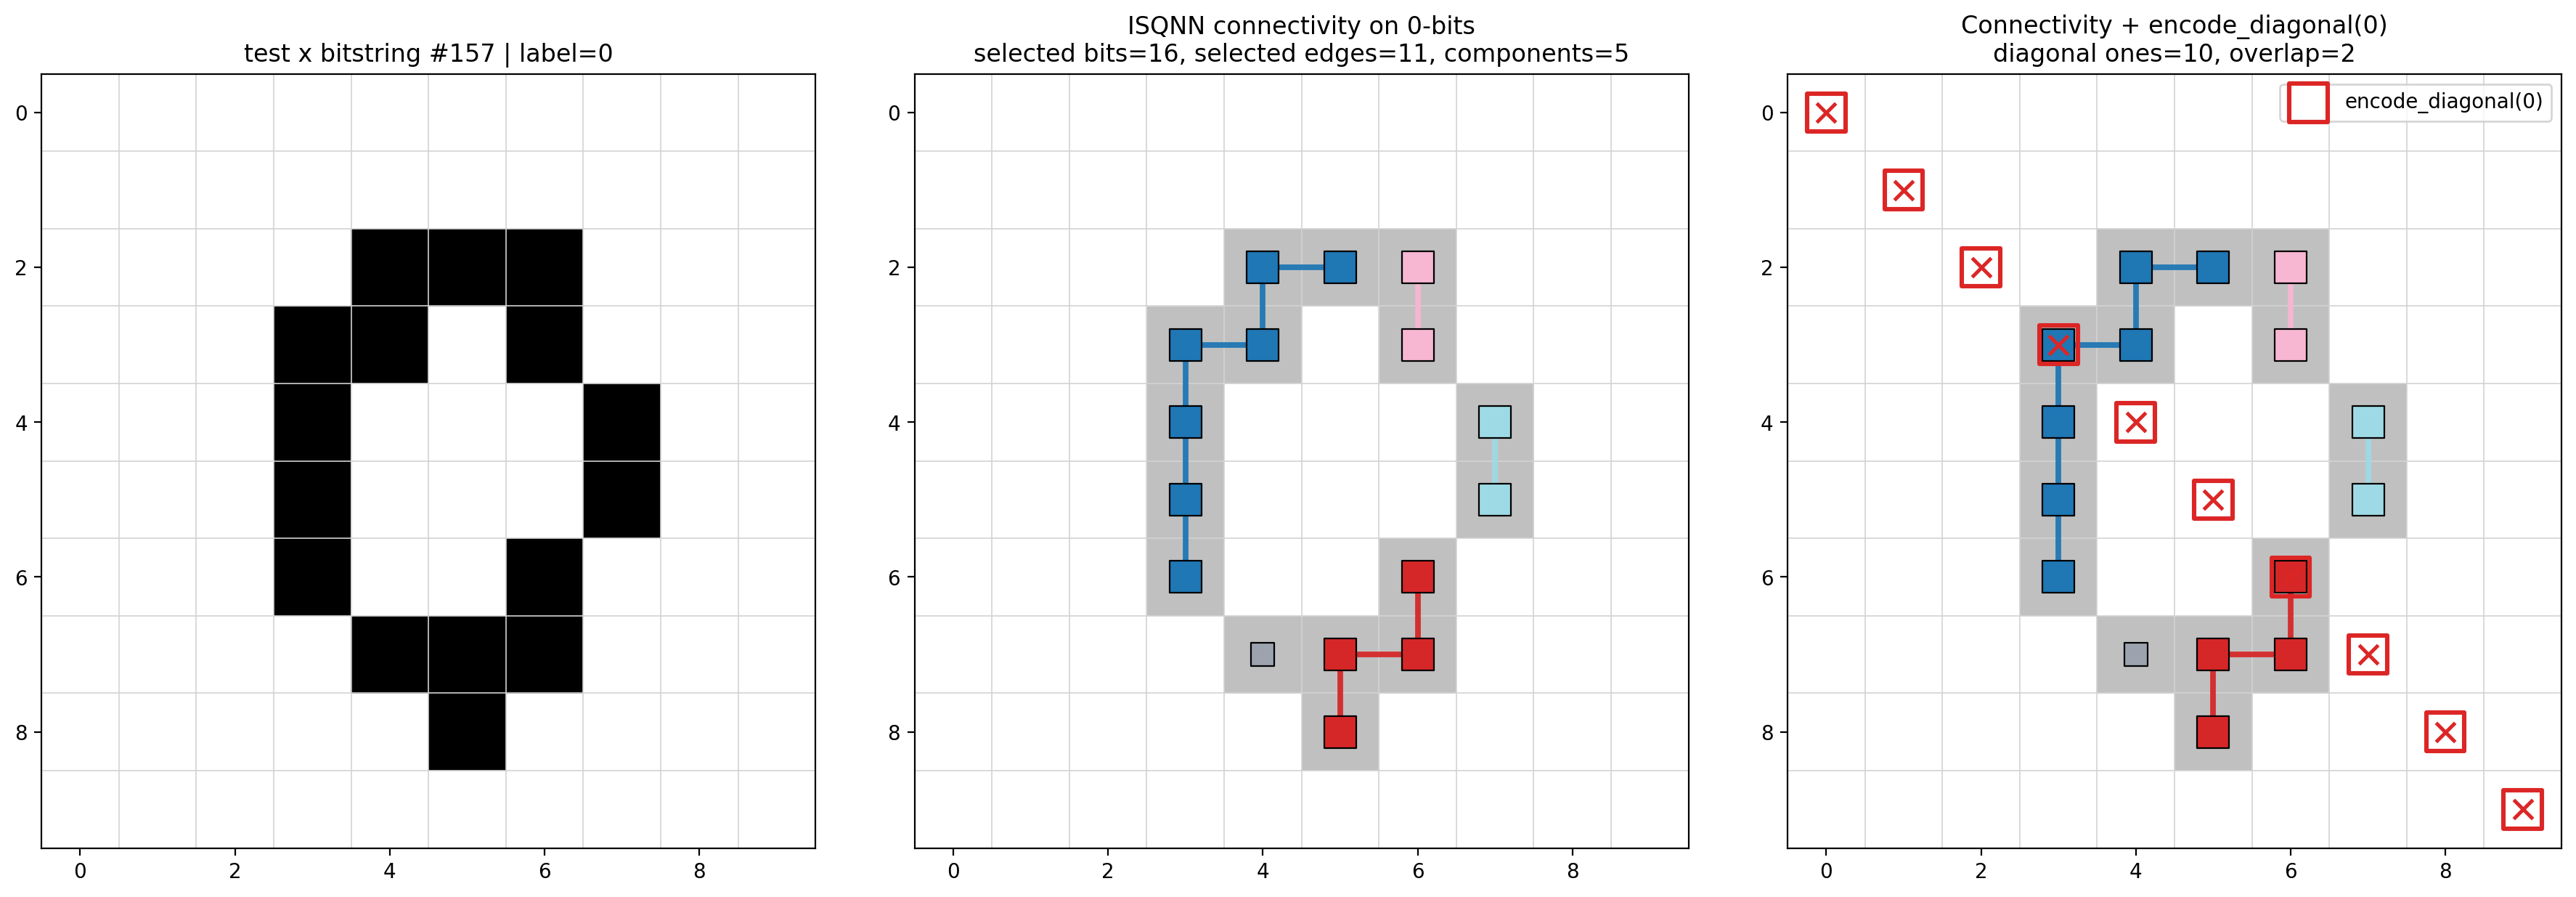
\includegraphics[width=0.96\textwidth,height=0.78\textheight,keepaspectratio]{mnist_test_157_connectivity_label_0.png}

  \vspace{0.25em}
  \footnotesize
  % The active qubits again split into multiple local components instead of one global object.
\end{frame}

\begin{frame}{Connectivity Example: Test Sample \#164}
  \centering
  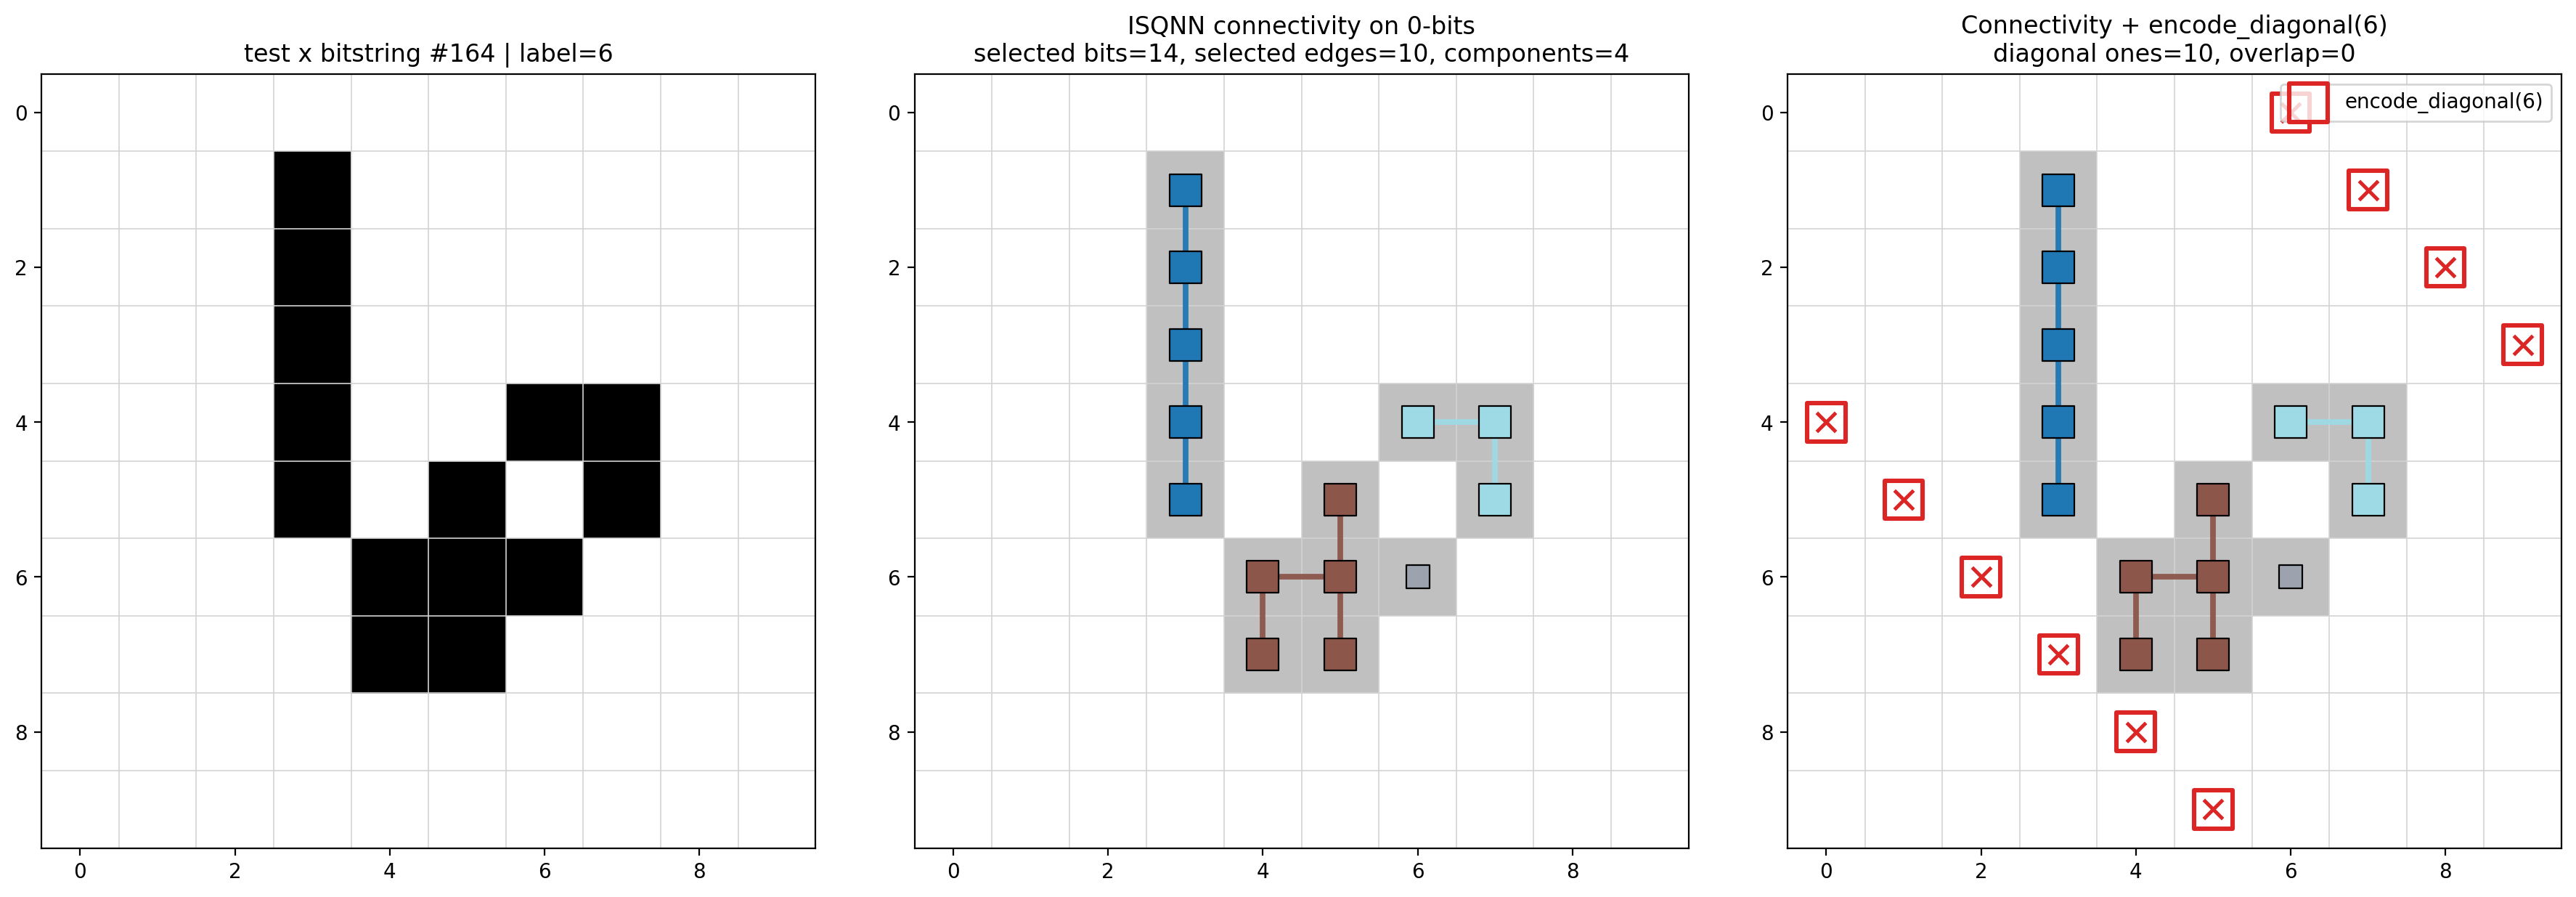
\includegraphics[width=0.96\textwidth,height=0.78\textheight,keepaspectratio]{mnist_test_164_connectivity_label_6.png}

  \vspace{0.25em}
  \footnotesize
  % Even when the sample shape changes, the same locality pattern remains.
\end{frame}

\begin{frame}{Factorized Output Family}
  \small
  For a fixed input pattern $x$:
  \[
    P(y\mid x,\theta)
    =
    2^{-|\mathcal W(x)|}
    \prod_{C\in \mathcal C(x)}
    P_C(y_C\mid \theta_C),
  \]
  where $\mathcal W(x)$ are pixels encoded to $\ket{0}$ and $\mathcal C(x)$ are CZ-connected components on pixels encoded to $\ket{+}$.

  \vspace{0.4em}
  \begin{itemize}
    \item White pixels contribute only uniform $50/50$ outputs in the $X$ basis.
    \item Nontrivial correlations exist only inside connected black-pixel blocks.
    \item Different blocks multiply independently.
  \end{itemize}
\end{frame}

\begin{frame}{Implication for Encoded Labels}
  \centering
  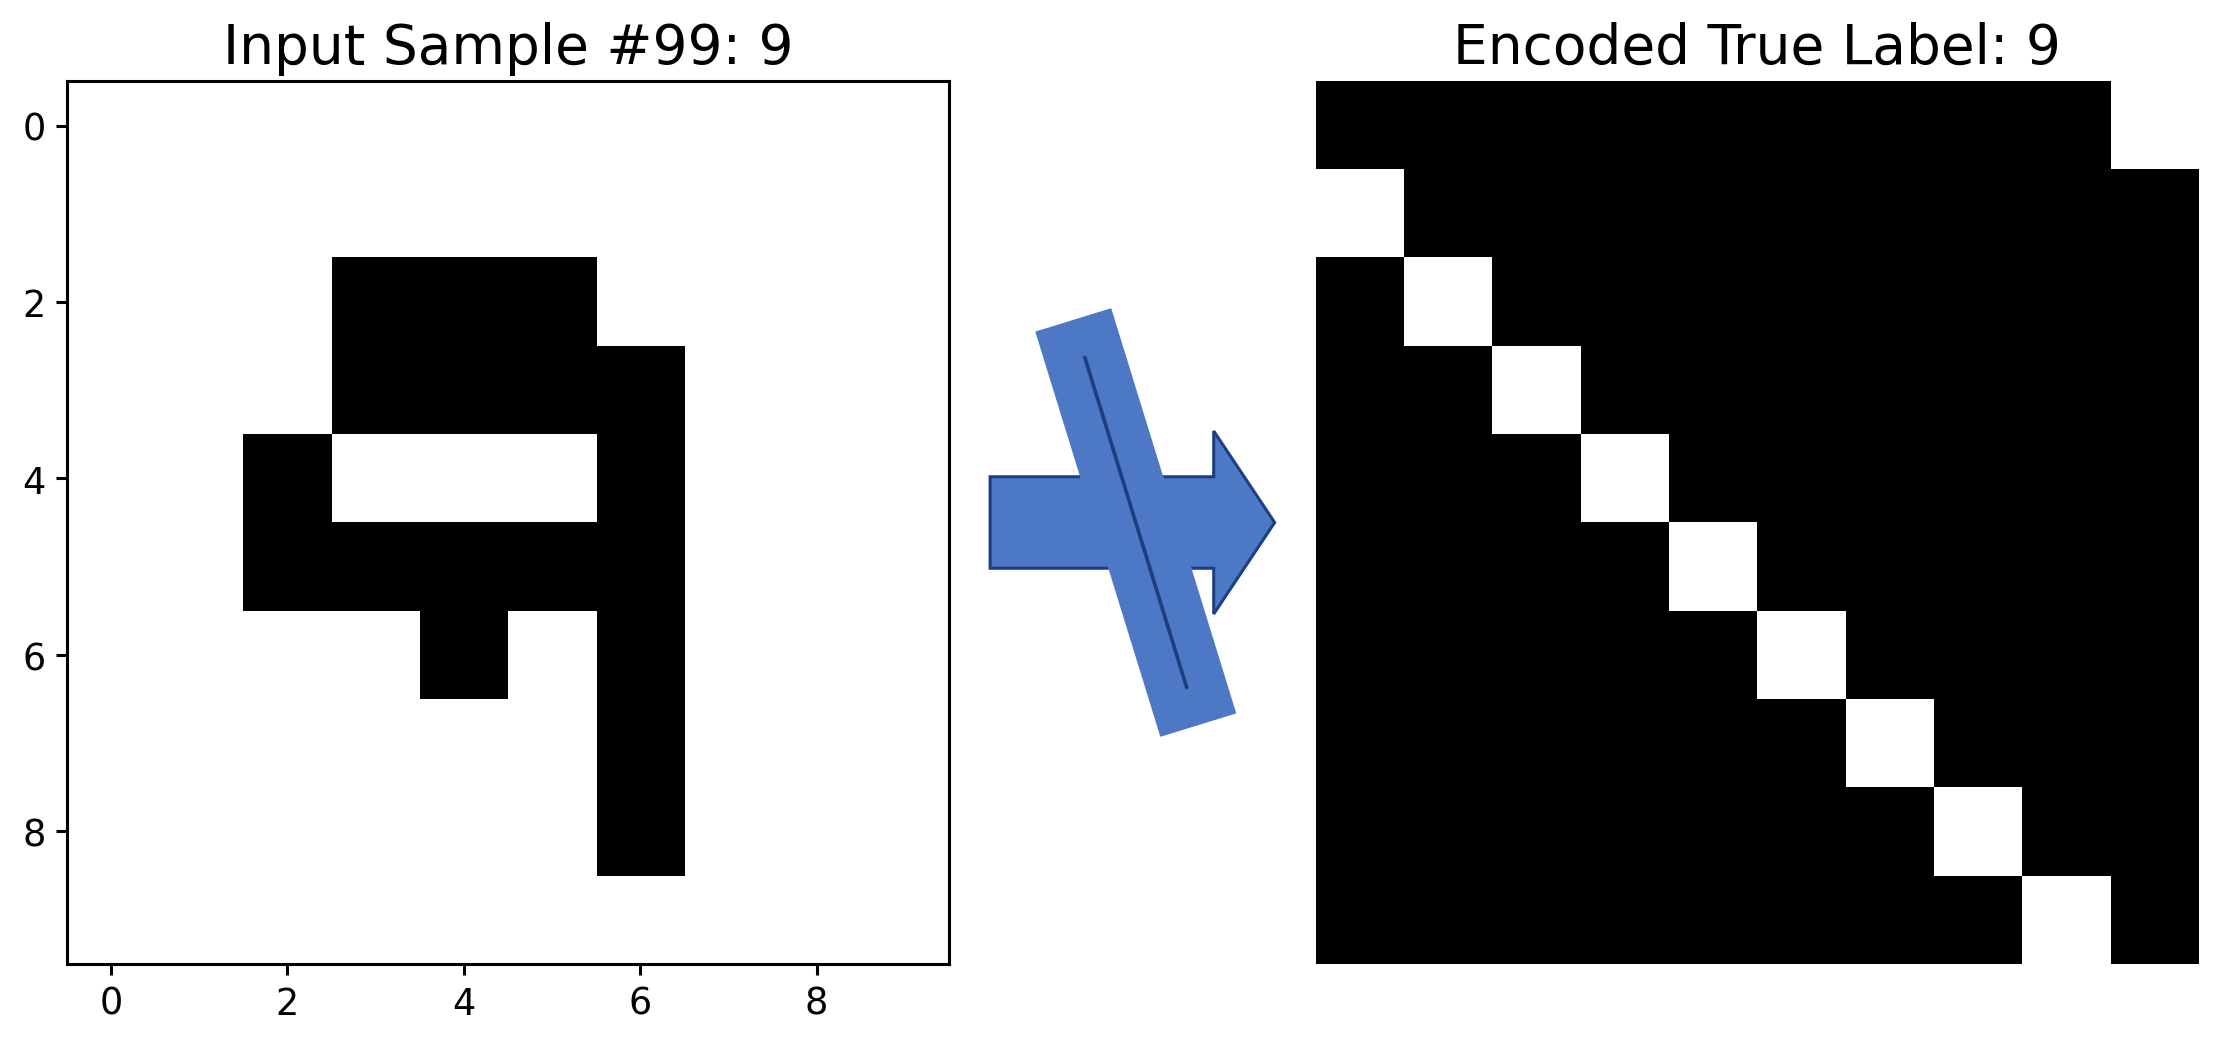
\includegraphics[width=0.78\textwidth,height=0.46\textheight,keepaspectratio]{sample99_vs_encoded_label_failure.png}

  \vspace{0.5em}
  \small
  \begin{itemize}
    \item The pre-encoded label is a global target pattern, but the IDQNN output for a handwritten-digit input is only a product of local connected-block distributions and uniform white-pixel noise.
  \end{itemize}
  
  \vspace{0.5em}
  \begin{alertblock}{Structural Limitation}
    Therefore IDQNN is structurally unable to reproduce any global pre-encoded label as a generic inference target for MNIST handwritten digits.
  \end{alertblock}
\end{frame}

\end{document}
